\documentclass[a4paper]{article}
\usepackage[utf8]{inputenc}
\usepackage{amsmath,amssymb}

\usepackage{indentfirst}
\usepackage{caption}

%\usepackage{tempora}
\usepackage{fontenc}
\usepackage[english, russian]{babel}
\usepackage[normalem]{ulem}

\usepackage[top=2cm, left=3cm, right=1.5cm, bottom=2cm]{geometry}
\usepackage{subfig}
\usepackage{listings}
\usepackage{wrapfig}
\usepackage{unnumberedtotoc}

\usepackage{amssymb}
\usepackage{amsmath}
\usepackage[pdftex]{graphicx}

\usepackage{fontsize}
  \changefontsize[12.8pt]{12pt}

\begin{document}


%
% ─── HEADER PAGE ────────────────────────────────────────────────────────────────
%

\begin{titlepage}

\begin{center}
\large \textbf{ БЕЛОРУССКИЙ ГОСУДАРСТВЕННЫЙ УНИВЕРСИТЕТ }\\
Факультет радиофизики и компьютерных технологий
\end{center}

\vspace{8em}

\Large
\huge
\begin{center}
\textbf{Реферат}
\end{center}

\Large
\begin{center}
Теоретические основы численных методов реализованных в лабораторном практикуме
\end{center}

\vspace{10em}


\hfill \parbox{10em}{
    Преподаватель:\newline
    Мулярчик Степан Григорьевич\newline

    Подготовил:\newline
    Глеба Евгений Михайлович\newline
    2 курс, АРИСТ,\newline
    4 группа
}



\vspace{\fill}

\begin{center}
Минск, 2022
\end{center}

\end{titlepage}

\setcounter{page}{2}


\tableofcontents

\newpage

\begin{center}
    \item \section{ РЕШЕНИЕ СИСТЕМ ЛИНЕЙНЫХ АЛГЕБРАИЧЕСИХ УРАВНЕНИЙ }
\end{center}

\subsection{Метод Гаусса}

Метод  Гаусса – наиболее мощный и универсальный инструмент для нахождения решения любой системы линейных уравнений. Как мы помним, правило Крамера и матричный метод непригодны в тех случаях, когда система имеет бесконечно много решений или несовместна. А метод последовательного исключения неизвестных в любом случае приведет нас к ответу.

Из прямых методов популярным у вычислителей является этот метод. Поиск главного элемента позволяет, с одной стороны, ограничить рост коэффициентов на каждом шаге исключения и, следовательно, уменьшить влияние ошибок округления на точность решения, с другой, обеспечить для невырожденных систем выполнение условия $a_{kk} \neq 0$ (отсутствие аварийных остановов вследствие деления на нуль).

Пусть исходная матрица выглядит так:

\begin{equation}
    \label{eqn:1.1}
    \begin{aligned}
    \begin{cases}
        & a_{11} x_{1}+a_{12} x_{2}+\cdots+a_{1 n} x_{n}=b_{1}, \\
        & a_{21} x_{1}+a_{22} x_{2}+\cdots+a_{2 n} x_{n}=b_{2}, \\
        & \cdots \\
        & a_{n 1} x_{1}+a_{n 2} x_{2}+\cdots+a_{n n} x_{n}=b_{n} .
    \end{cases}
    \end{aligned}
\end{equation}

Процесс её решения делится на два этапа, называемых соответственно прямым и обратным ходом.

На первом этапе система $(\ref{eqn:1.1})$ путем последовательного исключения переменных $x_{1}, x_{2}, \ldots, x_{n}$ сводится к эквивалентной системе с верхней треугольной матрицей коэффициентов с единичной диагональю:

\begin{equation}
    \label{eqn:1.2}
    \begin{aligned}
        \begin{array}{r}
            x_{1}+u_{12} x_{2}+u_{13} x_{3}+\cdots+u_{1, n-1} x_{n-1}+u_{1 n} x_{n}=q_{1}, \\
            x_{2}+u_{23} x_{3}+\cdots+u_{2, n-1} x_{n-1}+u_{2 n} x_{n}=q_{2}, \\
            \ldots \\
            x_{n-1}+u_{n-1, n} x_{n}=q_{n-1}, \\
            x_{n}=q_{n} .
        \end{array}
    \end{aligned}
\end{equation}

Исключение переменной $x_{k}$ (k-ый шаг прямого хода Гаусса) включает вычисление k-ой строки треугольной матрицы:

\begin{equation}
    \label{eqn:1.3}
    \begin{aligned}
        u_{k j}=a_{k j}^{(k-1)} / a_{k k}^{(k-1)}, j=\overline{k+1, n},
    \end{aligned}
\end{equation}

$\mathrm{k}$-го свободного члена:

\begin{equation}
    \label{eqn:1.4}
    \begin{aligned}
        q_{k}=b_{k}^{(k-1)} / a_{k k}^{(k-1)},
    \end{aligned}
\end{equation}

преобразование уравнений системы $(\ref{eqn:1.1})$ с номерами $\mathrm{k}+1, \mathrm{k}+2, \ldots, \mathrm{n}$ :

\begin{equation}
    \label{eqn:1.5}
    \begin{aligned}
        \begin{gathered}
            a_{i j}^{(k)}=a_{i j}^{(k-1)}-a_{i k}^{(k-1)} u_{k j} ; b_{i}^{(k)}=b_{i}^{(k-1)}-a_{i k}^{(k-1)} q_{k}, \\
            i=\overline{k+1, n} ; \ j=\overline{k+1, n} .
        \end{gathered}
    \end{aligned}
\end{equation}

На втором этапе (обратный ход) решают систему $(\ref{eqn:1.2})$:

\begin{equation}
    \label{eqn:1.6}
    \begin{aligned}
        \begin{gathered}
            x_{n}=q_{n} ; \quad x_{k}=q_{k}-\sum_{j=k+1}^{n} u_{k j} x_{j} ; \quad k=\overline{n-1,1},
        \end{gathered}
    \end{aligned}
\end{equation}

последовательно определяя неизвестные $x_{n}, x_{n-1, \ldots,} x_{1}$.

Метод Гаусса для плохо обусловленных матриц коэффициентов является вычислительно неустойчивым. Уменьшить вычислительную ошибку можно с помощью метода Гаусса с выделением главного элемента, который является условно устойчивым. Широкое применение метода Гаусса связано с тем, что плохо обусловленные матрицы встречаются на практике относительно редко.

\subsubsection{Алгоритм}

Алгоритм решения СЛАУ методом Гаусса подразделяется на два этапа:
\begin{itemize}
 \item На первом этапе осуществляется так называемый прямой ход, когда путём элементарных преобразований над строками систему приводят к ступенчатой или треугольной форме, либо устанавливают, что система несовместна. Для этого среди элементов первого столбца матрицы выбирают ненулевой, перемещают содержащую его строку в крайнее верхнее положение, делая эту строку первой. Далее ненулевые элементы первого столбца всех нижележащих строк обнуляются путём вычитания из каждой строки первой строки, домноженной на отношение первого элемента этих строк к первому элементу первой строки. После того, как указанные преобразования были совершены, первую строку и первый столбец мысленно вычёркивают и продолжают, пока не останется матрица нулевого размера. Если на какой-то из итераций среди элементов первого столбца не нашёлся ненулевой, то переходят к следующему столбцу и проделывают аналогичную операцию.

 \item На втором этапе осуществляется так называемый обратный ход, суть которого заключается в том, чтобы выразить все получившиеся базисные переменные через небазисные и построить фундаментальную систему решений, либо, если все переменные являются базисными, то выразить в численном виде единственное решение системы линейных уравнений. Эта процедура начинается с последнего уравнения, из которого выражают соответствующую базисную переменную (а она там всего одна) и подставляют в предыдущие уравнения, и так далее, поднимаясь по «ступенькам» наверх. Каждой строчке соответствует ровно одна базисная переменная, поэтому на каждом шаге, кроме последнего (самого верхнего), ситуация в точности повторяет случай последней строки.
\end{itemize}

Метод Гаусса требует $\mathrm{O}(n^3 / 3)$ арифметических операций.

\subsubsection{Реализация алгоритма на языке C\#}

\lstinputlisting[language=java, frame=single, caption=Метод Гаусса на языке C\#, tabsize=1, breaklines]{code/listing-1-1.cs}

\subsubsection{Применение и модификации}

Помимо аналитического решения СЛАУ, метод Гаусса также применяется для:

\begin{itemize}
 \item нахождения матрицы, обратной к данной (к матрице справа приписывается единичная такого же размера, что и исходная: $[A | E]$, после чего $A$ приводится к виду единичной матрицы методом Гаусса—Жордана; в результате на месте изначальной единичной матрицы справа оказывается обратная к исходной матрица: $[E | A^{-1}]$
 \item определения ранга матрицы (согласно следствию из теоремы Кронекера — Капелли ранг матрицы равен числу её главных переменных)
 \item численного решения СЛАУ в технических приложениях (для уменьшения погрешности вычислений используется Метод Гаусса с выделением главного элемента, суть которого заключена в том, чтобы на каждом шаге в качестве главной переменной выбирать ту, при которой среди оставшихся после вычёркивания очередных строк и столбцов стоит максимальный по модулю коэффициент).
\end{itemize}

\subsubsection{Достоинства метода}

\begin{itemize}
 \item Для матриц ограниченного размера — менее трудоёмкий по сравнению с другими методами.
 \item Позволяет однозначно установить, совместна система или нет, и если совместна, найти её решение.
 \item Позволяет найти максимальное число линейно независимых уравнений — ранг матрицы системы.
\end{itemize}

\subsubsection{Устойчивость метода Гаусса}

Метод Гаусса для плохо обусловленных матриц коэффициентов является вычислительно неустойчивым. Например, для матриц Гильберта метод приводит к очень большим ошибкам даже при небольшой размерности этих матриц. Уменьшить вычислительную ошибку можно с помощью метода Гаусса с выделением главного элемента, который является условно устойчивым. Широкое применение метода Гаусса связано с тем, что плохо обусловленные матрицы встречаются на практике относительно редко.

\subsubsection{Неоптимальность метода Гаусса}

В 1969 году Штрассен доказал, что большие матрицы можно перемножить за время $O(n^{log_2 7}) = O(n^{2.81})$. Отсюда вытекает, что обращение матриц и решение СЛАУ можно осуществлять алгоритмами асимптотически более быстрыми по порядку, чем метод Гаусса. Таким образом, для больших СЛАУ метод Гаусса не оптимален по скорости.

\subsection{Метод $\bar{L} D \bar{L}^{T}-$ факторизации}

Иногда удобнее бывает рассматривать $\bar{L} D \bar{L}^{T}$  вариант симметричного треугольного разложения, в котором матрица $L$ является нижней унитреугольной (т.е. имеет единицы на главной диагонали), а $D$ - диагональная матрица с положительными элементами.

Здесь мы опишем методы, использующие специфику при решении задачи
\(Ax = b\). В случае, когда \(A\) --- симметричная невырожденная
матрица, т.е. \(A = A^T\) и \(\det(A) \ne 0\), существует разложение
вида:

\begin{equation}
    \label{eqn:1.7}
    A = L D L^T,
\end{equation}


 где \(L\) --- нижняя унитреугольная матрица, \(D\) --- диагональная
матрица. В связи с этим работа связанная с получением разложения
:eq:\(sles-ldl\), составляет половину от того, что требуется для
исключения Гаусса. Когда разложение :eq:\(sles-ldl\) получено, решение
системы \(Ax = b\) может быть найдено посредством решения систем
\(Ly = b\) (прямая подстановка), \(Dz = y\) и \(L^T x = z\).

\subsubsection{\texorpdfstring{\(LDL^T\)-разложение}{LDL\^{}T-разложение}}\label{sles:direct:ld:ldl}

Разложение $(\ref{eqn:1.7})$ может быть найдено при
помощи исключения Гаусса, вычисляющего \(A = LU\), c последующим
определением \(D\) из уравнения \(U = DL^T\). Тем не менее можно
использовать интересный альтернативный алгоритм непосредственного
вычисления \(L\) и \(D\).

Допустим, что мы знаем первые \(j-1\) столбцов матрицы \(L\),
диагональные элементы \(d_1, d_2, \ldots, d_{j-1}\) матрицы \(D\) для
некоторого \(j\), \(1 \leq j \leq n\). Чтобы получить способ вычисления
\(l_{ij}\), \(i = j+1, j+2, \ldots, n\), и \(d_j\) приравняем \(j\)-е
столбцы в уравнении \(A = LDL^T\). В частности,

\begin{equation}
    \label{eqn:1.8}
    A(1:j,j) = Lv,
\end{equation}

где
\begin{center}
 $v = DL^T e_j = \begin{bmatrix}
   d_1 l_{j1}\\
   \vdots \\
   d_{j-1} l_{jj-1}\\
   d_j
   \end{bmatrix}$
\end{center}

Следовательно, компоненты \(v_k\), \(k = 1, 2, \ldots, j-1\) вектора
\(v\) могут быть получены простым масштабированием элементов \(j\)-й
строки матрицы \(L\). Формула для \(j\)-й компоненты вектора \(v\)
получается из \(j\)-го уравнения системы \(L(1:j, 1:j) v = A(1:j, j)\):

\[
   v_j = a_{jj} - \sum_{k = 1}^{j-1} l_{ik}v_k,
\] Когда мы знаем \(v\), мы вычисляем \(d_j = v_j\). «Нижняя» половина
формулы $(\ref{eqn:1.8})$ дает уравнение \[
   L(j+1:n, 1:j) v(1:j) = A(j+1:n, j),
\] откуда для вычисления \(j\)-го столбца матрицы \(L\) имеем: \[
   L(j+1:n, j) = (A(j+1:n,j) - L(j+1:n, 1:j-1)v(1:j-1))/v_j.
\]

\subsubsection{Реализация на языке Python}

Для получения \(LDL^T\)-разложения матрицы \(A\) можем написать функцию:

\lstinputlisting[language=python, frame=single, caption=$LDL^{T}$ разложение на языке python, tabsize=1, breaklines]{code/listing-1-2.py}

В этой реализации мы использовали векторизованные вычисления. Разберем
некоторые выражения. Строка

\begin{verbatim}
v[:j] = LD[j,:j]*LD[range(j),range(j)]
\end{verbatim}

заменяется следующим циклом:

\begin{verbatim}
for i in range(j):
    v[i] = LD[j,i]*LD[i,i]
\end{verbatim}

В нашей программе доступ к \texttt{j} диагональным элементам массива
\texttt{A} осуществляется выражением \texttt{A{[}range(j),range(j){]}}.

При вычислении \texttt{v{[}j{]}} использовалась функция \texttt{np.dot},
которая вычисляет скалярное произведение векторов.

тметим также строку

\begin{verbatim}
LD[j+1:,j] = (LD[j+1:,j] - np.dot(LD[j+1:,:j],v[:j]))/v[j]
\end{verbatim}

в которой используется срез \texttt{L{[}j+1:,j{]}}, т.е. элементы с
\texttt{j+1}-го до последнего в \texttt{j}-ом столбце.

Для решения системы \(Ax = b\)` с использованием \(LDL^T\)-разложения
можно написать следующую функцию:

\lstinputlisting[language=python, frame=single, caption=Решение $LDL^{T}$ системы на языке python, tabsize=1, breaklines]{code/listing-1-3.py}


\newpage

\begin{center}
 \section{РЕШЕНИЕ СИСТЕМ НЕЛИНЕЙНЫХ АЛГЕБРАИЧЕСКИХ УРАВНЕНИЙ}
\end{center}

Метод Ньютона, алгоритм Ньютона (также известный как метод касательных) — это итерационный численный метод нахождения корня (нуля) заданной функции. Метод был впервые предложен английским физиком, математиком и астрономом Исааком Ньютоном (1643—1727). Поиск решения осуществляется путём построения последовательных приближений и основан на принципах простой итерации. Метод обладает квадратичной сходимостью. Модификацией метода является метод хорд и касательных. Также метод Ньютона может быть использован для решения задач оптимизации, в которых требуется определить ноль первой производной либо градиента в случае многомерного пространства.

\subsection{Описание метода}

Чтобы численно решить уравнение {\(f(x) = 0\)}, его необходимо привести к эквивалентному уравнению:
{{\(x = \varphi(x)\)}, где {{\(\varphi\)} - сжимающее отображение.

Для наилучшей сходимости метода в точке очередного приближения {{\(x^{\ast}\)} должно выполняться условие
{{\(\varphi^{\prime}(x^{\ast}) = 0\)} Решение данного уравнения ищут в виде {{\(\varphi(x) = x + \alpha(x)f(x)\)} тогда:

\begin{equation}
\label{eqn:2.1}
    \begin{aligned}
            \varphi^{\prime}(x^{*})=1+\stackrel{}{\alpha^{\prime}}(x^{*})f(x^{*})+\alpha(x^{*})f^{\prime}(x^{*})=0
    \end{aligned}
\end{equation}

В предположении, что точка приближения «достаточно близка» к корню
{{\(\overset{\sim}{x}\)} и что заданная функция
{{\((f(x^{\ast}) \approx f(\overset{\sim}{x}) = 0)\)}
окончательная формула для
{{\(\alpha(x)\)}
такова:

\begin{equation}
\label{eqn:2.1}
    \begin{aligned}
            \alpha(x)=-{\frac{1}{f^{\prime}(x)}}
    \end{aligned}
\end{equation}

С учётом этого функция {{\(\varphi(x)\)} определяется:

\begin{equation}
\label{eqn:2.1}
    \begin{aligned}
            \varphi(x)=x-{\frac{f(x)}{f^{\prime}(x)}}
    \end{aligned}
\end{equation}

При некоторых условиях эта функция в окрестности корня осуществляет
сжимающее отображение.

\subsubsection{Доказательство}

Пусть дана вещественного переменного дважды непрерывно дифференцируемая в своей области
определения, производная которой нигде не обращается в нуль:

\begin{center}
 {{\(f(x):\mathbb{X}\rightarrow\mathbb{R},\; f(x) \in C^{2}(\mathbb{X});\quad\forall x \in \mathbb{X}\; f^{\prime}(x) \neq 0.\)}}
\end{center}

И необходимо доказать, что функция {{\(\varphi(x) = x - \frac{f(x)}{f^{\prime}(x)}\)}}
осуществляет сжимающее отображение вблизи корня уравнения
{\(f(x) = 0\)}.

В силу непрерывной дифференцируемости} функции {\(f(x)\)} и неравенства нулю её первой производной {\(\varphi(x)\)} непрерывна.

Производная {\(\varphi^{\prime}(x)\)} равна:

\begin{center}
 {\(\varphi^{\prime}(x) = \frac{f(x)f^{''}(x)}{\left( {f^{\prime}(x)} \right)^{2}}.\)}
\end{center}

В условиях, наложенных на
{\(f(x)\)}, она также непрерывна. Пусть {\(\overset{\sim}{x}\)}
искомый корень уравнения: {\(f(\overset{\sim}{x}) = 0\)},
следовательно в его окрестности {\(\varphi^{\prime}(x) \approx 0\)}:

\begin{center}
 {\(\forall\varepsilon:0 < \varepsilon < 1,\;\exists\delta > 0\;\forall x \in \mathbb{X}\;|x - \overset{\sim}{x}| < \delta:|\varphi^{\prime}(x) - 0| < \varepsilon.\)}
\end{center}

Тогда согласно теореме Лагранжа:

\begin{center}
 {\(\forall x_{1},\; x_{2} \in U_{\delta}(\overset{\sim}{x})\;\exists\xi \in U_{\delta}(\overset{\sim}{x}):|\varphi(x_{1}) - \varphi(x_{2})| = |\varphi^{\prime}(\xi)||x_{1} - x_{2}| < \varepsilon|x_{1} - x_{2}|.\)}
\end{center}

В силу того, что {\(\varphi(\overset{\sim}{x}) = \overset{\sim}{x}\)} в этой же дельта окрестности выполняется:

\begin{center}
 {\(\forall x \in U_{\delta}(\overset{\sim}{x}):\;|\varphi(x) - \overset{\sim}{x}| < \varepsilon|x - \overset{\sim}{x}|.\)}
\end{center}

Таким образом полученная функция {\(\varphi(x)\)} в окрестности корня {\(U_{\delta}(\overset{\sim}{x})\)} осуществляет сжимающее отображение.


Поэтому алгоритм нахождения численного решения уравнения {\(f(x) = 0\)} сводится к итерационной процедуре вычисления:

\begin{center}
 {\(x_{n + 1} = x_{n} - \frac{f(x_{n})}{f^{\prime}(x_{n})}.\)}
\end{center}

По теореме Банаха последовательность приближений стремится к корню уравнения {\(f(x) = 0\)}.

\begin{figure}[h]
 \begin{center}
  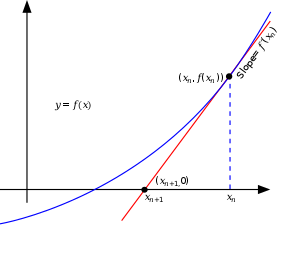
\includegraphics[width=3.125in,height=2.70833in]{images/Newton_iteration.png}
 \end{center}
  \caption{\textit{Иллюстрация метода Ньютона (синим изображена функция {\(f(x)\)},
    ноль которой необходимо найти, красным - касательная в точке
    очередного приближения {\(x_{n}\)}
    Здесь мы можем увидеть, что последующее приближение {\(x_{n + 1}\)}
    лучше предыдущего {\(x_{n}\)}.}}
\end{figure}


\subsubsection{Ограничения}

Пусть задано уравнение {{\(f(x) = 0\)}}, где
{{\(f(x):\mathbb{X}\rightarrow\mathbb{R}\)}} и надо найти его решение.

Ниже приведена формулировка основной теоремы, которая позволяет дать
чёткие условия применимости. Она носит имя советского и (---).

\textbf{Теорема Канторовича.}

\emph{Если существуют такие константы {{\(A,\; B,\; C\)}}, что:}

\begin{enumerate}
\item
  \emph{{{\(\frac{1}{|f^{\prime}(x)|} < A\)}} на
  {{\(\lbrack a,\; b\rbrack\)}}, то есть {{\(f^{\prime}(x)\)}}
  существует и не равна нулю;}
\item
  \emph{{{\(\left| \frac{f(x)}{f^{\prime}(x)} \right| < B\)}} на
  {{\(\lbrack a,\; b\rbrack\)}}, то есть {{\(f(x)\)}} ограничена;}
\item
  \emph{{{\(\exists f^{''}(x)\)}} на {{\(\lbrack a,\; b\rbrack\)}}, и
  {{\(|f^{''}(x)| \leqslant C \leqslant \frac{1}{2AB}\)}};}
\end{enumerate}

\emph{Причём длина рассматриваемого отрезка
{{\(|a - b| < \frac{1}{AB}\left( {1 - \sqrt{1 - 2ABC}} \right)\)}}.
Тогда справедливы следующие утверждения:}

\begin{enumerate}
\item
  \emph{на {{\(\lbrack a,\; b\rbrack\)}} существует корень
  {{\(x^{\ast}\)}} уравнения
  {{\(f(x) = 0:\exists x^{\ast} \in \lbrack a,\; b\rbrack:f(x^{\ast}) = 0\)}};}
\item
  \emph{если {{\(x_{0} = \frac{a + b}{2}\)}}, то итерационная сходится к
  этому корню:
  {{\(\left\{ {x_{n + 1} = x_{n} - \frac{f(x_{n})}{f^{\prime}(x_{n})}} \right\}\rightarrow x^{\ast}\)}};}
\item
  \emph{погрешность может быть оценена по формуле
  {{\(|x^{\ast} - x_{n}| \leqslant \frac{B}{2^{n - 1}}(2ABC)^{2^{n - 1}}\)}}.}
\end{enumerate}

Из последнего из утверждений теоремы в частности следует квадратичная
метода:

{{\(|x^{\ast} - x_{n}| \leqslant \frac{B}{2^{n - 1}}(2ABC)^{2^{n - 1}} = \frac{1}{2}\frac{B}{2^{n - 2}}\left( {(2ABC)^{2^{n - 2}}} \right)^{2} = \alpha|x^{\ast} - x_{n - 1}|^{2}.\)}}

Тогда ограничения на исходную функцию {{\(f(x)\)}} будут выглядеть так:

\begin{enumerate}
\item
  функция должна быть ограничена;
\item
  функция должна быть , дважды ;
\item
  её первая {{\(f^{\prime}(x)\)}} равномерно отделена от нуля;
\item
  её вторая производная {{\(f^{''}(x)\)}} должна быть равномерно
  ограничена.
\end{enumerate}

\subsection{Обобщения и модификации}
\subsubsection{Многомерный случай}
Обобщим полученный результат на многомерный случай.

Пусть необходимо найти решение системы:

\begin{center}
    {\(\left\{ \begin{matrix}
    {f_{1}(x_{1},\; x_{2},\;\ldots,\; x_{n})} & = & {0,} \\
    \ldots & & \\
    {f_{m}(x_{1},\; x_{2},\;\ldots,\; x_{n})} & = & 0. \\
    \end{matrix} \right.\)}
\end{center}

Выбирая некоторое начальное значение {\({\overset{\rightarrow}{x}}^{\lbrack 0\rbrack}\)},
последовательные приближения {\({\overset{\rightarrow}{x}}^{\lbrack j + 1\rbrack}\)}
находят путём решения систем уравнений:

\begin{center}
 {\(f_{i} + \sum\limits_{k = 1}^{n}\frac{\partial f_{i}}{\partial x_{k}}(x_{k}^{\lbrack j + 1\rbrack} - x_{k}^{\lbrack j\rbrack}) = 0,\qquad i = 1,\; 2,\;\ldots,\; m,\)}
\end{center}

где

\begin{center}
 {\({\overset{\rightarrow}{x}}^{\lbrack j\rbrack} = (x_{1}^{\lbrack j\rbrack},\; x_{2}^{\lbrack j\rbrack},\;\ldots,\; x_{n}^{\lbrack j\rbrack}),\quad j = 0,\; 1,\; 2,\;\ldots\)}.
\end{center}

\subsubsection{Метод секущих}

Родственный является «приближённым» методом Ньютона и позволяет
\textbf{не вычислять} производную. Значение производной в итерационной
формуле заменяется её оценкой по двум предыдущим точкам итераций:

\begin{center}
 {{\(f^{\prime}(x_{n}) \approx \frac{f(x_{n}) - f(x_{n - 1})}{x_{n} - x_{n - 1}}\)}}
\end{center}

Таким образом, основная формула имеет вид
\begin{center}
 {{\(x_{n + 1} = x_{n} - f(x_{n}) \cdot \frac{x_{n} - x_{n - 1}}{f(x_{n}) - f(x_{n - 1})}.\)}}
\end{center}

Этот метод схож с методом Ньютона, но имеет немного меньшую скорость
сходимости. Порядок сходимости метода равен ~--- 1,618\ldots{}

\textbf{Замечания.} 1) Для начала итерационного процесса требуются два
различных значения {{\(x_{0}\)}} и {{\(x_{1}\)}} .\\
2) В отличие от «настоящего метода Ньютона» (метода касательных),
требующего хранить только {{\(x_{n}\)}} (и в ходе вычислений~---
временно {{\(f(x_{n})\)}} и {{\(f^{\prime}(x_{n})\)}}), для метода
секущих требуется сохранение {{\(x_{n - 1}\)}} , {{\(x_{n}\)}} ,
{{\(f(x_{n - 1})\)}} , {{\(f(x_{n})\)}} .\\
3) Применяется, если вычисление {{\(f^{\prime}(x)\)}} затруднено
(например, требует большого количества машинных ресурсов: времени и/или
памяти).

\subsubsection{Метод Ньютона - Рафсона}
Метод Ньютона~--- Рафсона является улучшением метода Ньютона нахождения
экстремума, описанного выше. Основное отличие заключается в том, что на
очередной итерации каким-либо из выбирается оптимальный шаг:

{{\({\overset{\rightarrow}{x}}^{\lbrack j + 1\rbrack} = {\overset{\rightarrow}{x}}^{\lbrack j\rbrack} - \lambda_{j}H^{- 1}({\overset{\rightarrow}{x}}^{\lbrack j\rbrack})\nabla f({\overset{\rightarrow}{x}}^{\lbrack j\rbrack}),\)}}

где
{{\(\lambda_{j} = \arg\min\limits_{\lambda}f({\overset{\rightarrow}{x}}^{\lbrack j\rbrack} - \lambda H^{- 1}({\overset{\rightarrow}{x}}^{\lbrack j\rbrack})\nabla f({\overset{\rightarrow}{x}}^{\lbrack j\rbrack})).\)}}
Для оптимизации вычислений применяют следующее улучшение: вместо того,
чтобы на каждой итерации заново вычислять, ограничиваются начальным
приближением {{\(H(f({\overset{\rightarrow}{x}}^{\lbrack 0\rbrack}))\)}}
и обновляют его лишь раз в {{\(m\)}} шагов, либо не обновляют вовсе.

\subsection{Алгоритм}

\begin{enumerate}
    \item Задается начальное приближение {\(x_{0}\)}.
    \item Пока не выполнено условие остановки, в качестве которого можно взять {\(|x_{n + 1} - x_{n}| < \varepsilon\)} или {\(|f(x_{n + 1})| < \varepsilon\)} (то есть погрешность в нужных пределах), вычисляют новое приближение: {\(x_{n + 1} = x_{n} - \frac{f(x_{n})}{f^{\prime}(x_{n})}\)}.
\end{enumerate}

\subsubsection{Реализация на языке Haskell}

\lstinputlisting[language=haskell, frame=single, caption=Метод Ньютона на языке $Haskell$, tabsize=1, breaklines]{code/listing-2-1.hs}

\newpage

\begin{center}
 \section{РЕШЕНИЕ СИСТЕМ ОБЫКНОВЕННЫХ ДИФФЕРЕНЦИАЛЬНЫХ УРАВНЕНИЙ}
\end{center}

\begin{wrapfigure}{l}{0.25\textwidth}
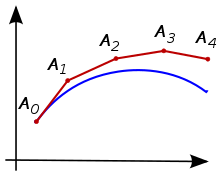
\includegraphics[width=0.9\linewidth]{images/Euler_method.png}
\caption{\textit{Ломаная Эйлера — приближённое решение в пяти узлах задачи Коши и точное решение этой задачи}}
\label{fig:wrapfig}
\end{wrapfigure}

Метод Эйлера~--- простейший численный метод решения систем обыкновенных дифференциальных уравнений. Впервые описан Леонардом Эйлером в 1768 году в работе «Интегральное исчисление». Метод Эйлера является явным, одношаговым методом первого порядка точности. Он основан на аппроксимации интегральной кривой кусочно-линейной функцией, так называемой ломаной Эйлера.

\subsection{Описание метода}

Пусть дана для уравнения первого порядка:
\begin{center}
    {{\(\frac{dy}{dx} = f(x,y),\)}}
    {{\(y_{|_{x = x_{0}}} = y_{0},\)}}
\end{center}

где функция {{\(f\)}} определена на некоторой области
{{\(D \subset \mathbb{R}^{2}\)}}. Решение ищется на полуинтервале
{{\((x_{0},b\rbrack\)}}. На этом промежутке введём узлы:
{{\(x_{0} < x_{1} < \cdots < x_{n} \leq b.\)}} Приближенное решение в
узлах {{\(x_{i}\)}}, которое обозначим через {{\(y_{i}\)}}, определяется
по формуле:

\begin{center}
 {{\(y_{i} = y_{i - 1} + (x_{i} - x_{i - 1})f(x_{i - 1},y_{i - 1}),\quad i = 1,2,3,\ldots,n.\)}}
\end{center}

Эти формулы непосредственно обобщаются на случай систем обыкновенных
дифференциальных уравнений.

\subsubsection{Оценка погрешности метода на шаге и в целом}

Погрешность на шаге или локальная погрешность~--- это разность между
численным решением после одного шага вычисления {{\(y_{i}\)}} и точным
решением в точке {{\(x_{i} = x_{i - 1} + h\)}}. Численное решение
задаётся формулой

\begin{center}
 {{\(y_{i} = y_{i - 1} + hf(x_{i - 1},y_{i - 1}).\quad\)}}
\end{center}

Точное решение можно разложить в :

\begin{center}
 {{\(y(x_{i - 1} + h) = y(x_{i - 1}) + hy^{\prime}(x_{i - 1}) + O(h^{2}).\)}}
\end{center}

Локальную ошибку {{\(L\)}} получаем, вычитая из второго равенства
первое:

\begin{center}
 {{\(L = y(x_{i - 1} + h) - y_{i} = O(h^{2}).\)}}
\end{center}

Это справедливо, если {{\(y\)}} имеет непрерывную вторую
производную\textsuperscript{}. Другим достаточным условием
справедливости этой оценки, из которого вытекает предыдущее и которое
обычно может быть легко проверено, является непрерывная
дифференцируемость {{\(f(x,y)\)}} по обоим аргументам\textsuperscript{}.

Погрешность в целом, глобальная или накопленная погрешность~--- это
погрешность в последней точке произвольного конечного отрезка
интегрирования уравнения. Для вычисления решения в этой точке требуется
{{\(S/h\)}} шагов, где {{\(S\)}} длина отрезка. Поэтому глобальная
погрешность метода {{\(G = O(h^{2}S/h) = O(h)\)}}.

Таким образом, метод Эйлера является методом первого порядка~--- имеет
погрешность на шаге {{\(O(h^{2})\)}} и погрешность в целом
{{\(O(h)\)}}\textsuperscript{}.

\subsection{Явный метод Эйлера}
Формула интегрирования явного метода Эйлера имеет вид:

$$
y_{k+1}=y_{k}+\tau_{k} f\left(y_{k}, t_{k}\right), \quad k=0,1,2, \ldots
$$

где $\tau_{\mathrm{k}}$ - шаг интегрирования. Его локальная погрешность

$$
\varepsilon_{k}=\frac{\tau_{k}^{2}}{2} u^{\prime \prime}(\tilde{t}) \quad \tilde{t} \in\left[t_{k} ; t_{k+1}\right]
$$

пропорциональна $\tau_{k}^{2}$, т. е. явный метод Эйлера имеет первый порядок точности. Приведем геометрическую интерпретацию явного метода Эйлера для задачи Коши: приращение на шаре интегрирования метода - катет значению производной в предыдущий момент времени. Вторым катетом этого треугольника является текущий шаг интегрирования.

Явный метод Эйлера для СОДУ является условно устойчивым с условием:

$$
\left|1+\tau \lambda_{i}\right|<1, i=\overline{1, n}
$$

где $\lambda_{i}-$ собственные числа матрицы $\mathrm{J}=\mathrm{df} / \mathrm{dx}$. Поэтому выбор величины шага интегрирования в явном методе Эйлера необходимо делать, исходя из сохранения устойчивости и точности вычислений.

Шаг мы вычисляем по формулам:

$$
\tau_{k}^{i}\leq\varepsilon_{i,0n}^{i}/ \big[|f^{i}(\mathbf{y}_{k},t_{k})|+\varepsilon_{n,0n}^{i}/\tau_{\mathrm{max}}\big]
$$

Из (3) вытекает:

$$
\tau_{k}=\min _{i=1, n} \tau_{k}^{i}
$$

\subsubsection{Реализация на языке Python}

\lstinputlisting[language=python, frame=single, caption=Явный метод Эйлера на языке Python, tabsize=1, breaklines]{code/listing-3-1.py}

\subsection{Неявный метод Эйлера}
Разностная схема неявного метода Эйлера выглядит следующим образом:

$$
\mathbf{y}_{k+1}=\mathbf{y}_{k}+\tau_{k} \mathbf{f}\left(\mathbf{y}_{k+1}, t_{k+1}\right), \quad k=0,1,2, \ldots
$$

Она требует на каждом временном шаге решения следующей алгебраической задачи:

$$
\mathbf{F}\left(\mathbf{y}_{k+1}\right)=\mathbf{y}_{k+1}-\mathbf{y}_{k}-\tau_{k} \mathbf{f}\left(\mathbf{y}_{k+1}, t_{k+1}\right)=0
$$

которую можно решить, например, методом Ньютона.

Локальная погрешность неявного метода Эйлера

$$
\varepsilon_{k}=-\frac{\tau_{k}^{2}}{2} u^{\prime \prime}(\tilde{t}) \quad \tilde{t} \in\left[t_{k} ; t_{k+1}\right]
$$

% \begin{center}
% \includegraphics[max width=\textwidth]{2022_12_16_a4190c38e0c8eb47c7ceg-07}
% \end{center}

по порядку величины $\tau \mathrm{k}$ является такой же, как и локальная погрешность явного метода Эйлера, и противоположна по знаку. После выполнения шага интегрирования $\tau_{k}$ вычисляются $\varepsilon_{k}^{i}$ по формуле $\varepsilon_{k}$ для всех переменных $u^{i}$. Если хотя бы одно $\left|\varepsilon_{k}^{i}\right|>\varepsilon_{\text {доп }}^{i}$ то шаг $\tau_{k}$ уменьшается вдвое, и вычисления повторяются.

При выборе шага интегрирования можно использовать также стратегию трёх зон:

% \begin{center}
% \includegraphics[max width=\textwidth]{2022_12_16_a4190c38e0c8eb47c7ceg-08}
% \end{center}

В обоих стратегиях окончательный шаг интегрирования выбирается минимальным среди всех значений $\tau_{k+1}^{i}$.

Неявный метод Эйлера является абсолютно устойчивым по отношению к шагу интегрирования. При решении этим методом жёстких систем дифференциальных уравнений шаг интегрирования выбирается только из соображений допустимой локальной погрешности.

\subsubsection{Реализация на языке Python}

\lstinputlisting[language=python, frame=single, caption=Неявный метод Эйлера на языке Python, tabsize=1, breaklines]{code/listing-3-2.py}

\subsection{Модификации и обобщения}

\subsubsection{Модифицированный метод Эйлера с пересчетом}

Повысить точность и устойчивость вычисления решения можно с помощью
явного метода Эйлера следующего вида.

Прогноз:
\begin{center}
 {{\({\overset{\sim}{y}}_{i} = y_{i - 1} + (x_{i} - x_{i - 1})f(x_{i - 1},y_{i - 1})\)}}.
\end{center}

Коррекция:

\begin{center}
 {{\(y_{i} = y_{i - 1} + (x_{i} - x_{i - 1})\frac{f(x_{i - 1},y_{i - 1}) + f(x_{i},{\overset{\sim}{y}}_{i})}{2}\)}}.
\end{center}


Для повышения точности корректирующую итерацию можно повторить,
подставляя {{\({\overset{\sim}{y}}_{i} = y_{i}\)}} .

Модифицированный метод Эйлера с пересчетом имеет второй порядок
точности, однако для его реализации необходимо как минимум дважды
вычислять {{\(f(x,y)\)}}. Метод Эйлера с пересчетом представляет собой
разновидность (предиктор-корректор).

\subsubsection{Двухшаговый метод Адамса~--- Башфорта}

Другой способ повысить точность метода заключается в использовании не
одного, а нескольких вычисленных ранее значений функции:

\begin{center}
 {{\(y_{i + 1} = y_{i} + \frac{3}{2}hf(x_{i},y_{i}) - \frac{1}{2}hf(x_{i - 1},y_{i - 1}).\)}}
\end{center}

Это линейный многошаговый метод.

\newpage

\begin{center}
 \section{ПРИБЛИЖЕНИЕ ФУНКЦИИ МЕТОДОМ НАИМЕНЬШИХ КВАДРАТОВ}
\end{center}

Метод наименьших квадратов (МНК) — математический метод, применяемый для решения различных задач, основанный на минимизации суммы квадратов отклонений некоторых функций от экспериментальных входных данных. Он может использоваться для «решения» переопределенных систем уравнений (когда количество уравнений превышает количество неизвестных), для поиска решения в случае обычных (не переопределенных) нелинейных систем уравнений, для аппроксимации точечных значений некоторой функции. МНК является одним из базовых методов регрессионного анализа для оценки неизвестных параметров регрессионных моделей по выборочным данным.

\subsection{Суть метода наименьших квадратов}

Пусть {{\(y_{i}\)}}, {{\(i = 1,...n\)}} набор скалярных
экспериментальных данных, {{\(x_{i}\)}}, {{\(i = 1,...n\)}} набор
векторных экспериментальных данных и предполагается, что {{\(y\)}}
зависит от {{\(x\)}}.

Вводится некоторая (в простейшем случае линейная) скалярная функция
{{\(f(x,\mathbf{\beta})\)}}, которая определяется вектором неизвестных
параметров {{\(\beta\)}}.

Ставится задача найти вектор {{\(\beta\)}} такой, чтобы совокупность
погрешностей {{\(r_{i} = y_{i} - f(x_{i},\mathbf{\beta})\)}} была в
некотором смысле минимальной.

Согласно методу наименьших квадратов решением этой задачи является
вектор {{\(\beta\)}}, который минимизирует функцию

\begin{center}
 {{\(S(\mathbf{\beta}) = \sum\limits_{i = 1}^{n}(y_{i} - f(x_{i},\mathbf{\beta}))^{2}.\)}}
\end{center}

В простейшем случае {{\(f(x) = \beta\)}}, и тогда результатом МНК будет
входных данных.

Преимущество МНК перед минимизацией других видов ошибок состоит в том,
что если {{\(f(x,\mathbf{\beta})\)}} дифференцируема по
{{\(\mathbf{\beta}\)}}, то {{\(S(\mathbf{\beta})\)}} тоже
дифференцируема. Приравнивание частных производных к нулю сводит задачу
к решению системы уравнений, причём если {{\(f(x,\mathbf{\beta})\)}}
зависит от {{\(\mathbf{\beta}\)}} линейно, то и система уравнений будет
линейной.

\subsection{МНК в регрессионном анализе (аппроксимация данных)}

Пусть имеется {{\(n\)}} значений некоторой переменной {{\(y\)}} (это
могут быть результаты наблюдений, экспериментов и~т.~д.) и
соответствующих переменных {{\(x\)}}. Задача заключается в том, чтобы
взаимосвязь между {{\(y\)}} и {{\(x\)}} аппроксимировать некоторой
функцией {{\(f(x,b)\)}}, известной с точностью до некоторых неизвестных
параметров {{\(b\)}}, то есть фактически найти наилучшие значения
параметров {{\(b\)}}, максимально приближающие значения {{\(f(x,b)\)}} к
фактическим значениям {{\(y\)}}. Фактически это сводится к случаю
«решения» переопределенной системы уравнений относительно {{\(b\)}}:

\begin{center}
 {{\(f(x_{t},b) = y_{t},t = 1,\ldots,n\)}}.
\end{center}


В регрессионном анализе и в частности в эконометрике используются
вероятностные модели зависимости между переменными

\begin{center}
 {{\(y_{t} = f(x_{t},b) + \varepsilon_{t}\)}},
\end{center}

где {{\(\varepsilon_{t}\)}}~--- так называемые \emph{случайные ошибки}
модели.

Соответственно, отклонения наблюдаемых значений {{\(y\)}} от модельных
{{\(f(x,b)\)}} предполагается уже в самой модели. Сущность МНК
(обычного, классического) заключается в том, чтобы найти такие параметры
{{\(b\)}}, при которых сумма квадратов отклонений (ошибок, для
регрессионных моделей их часто называют \emph{остатками регрессии})
{{\(e_{t}\)}} будет минимальной:

\begin{center}
 {{\({\hat{b}}_{OLS} = \arg\min\limits_{b}RSS(b)\)}},
\end{center}

где {{\(RSS\)}}~--- ~\foreignlanguage{english}{Residual Sum of
Squares}\textsuperscript{} определяется как:

\begin{center}
 {{\(RSS(b) = e^{T}e = \sum\limits_{t = 1}^{n}e_{t}^{2} = \sum\limits_{t = 1}^{n}(y_{t} - f(x_{t},b))^{2}\)}}.
\end{center}

В общем случае решение этой задачи может осуществляться численными
методами оптимизации (минимизации). В этом случае говорят о
\emph{нелинейном МНК} (NLS или NLLS~---
~\foreignlanguage{english}{Non-Linear Least Squares}). Во многих случаях
можно получить аналитическое решение. Для решения задачи минимизации
необходимо найти стационарные точки функции {{\(RSS(b)\)}},
продифференцировав её по неизвестным параметрам {{\(b\)}}, приравняв
производные к нулю и решив полученную систему уравнений:

\begin{center}
 {{\(\sum\limits_{t = 1}^{n}(y_{t} - f(x_{t},b))\frac{\partial f(x_{t},b)}{\partial b} = 0\)}}.
\end{center}

\subsubsection{МНК в случае линейной регрессии}

Пусть регрессионная зависимость является линейной:

\begin{center}
 {{\(y_{t} = \sum\limits_{j = 1}^{k}b_{j}x_{tj} + \varepsilon = x_{t}^{T}b + \varepsilon_{t}\)}}.
\end{center}

Пусть \emph{y}~--- вектор-столбец наблюдений объясняемой переменной, а
{{\(X\)}}~--- это {{\(({n \times k})\)}}-матрица наблюдений факторов
(строки матрицы~--- векторы значений факторов в данном наблюдении, по
столбцам~--- вектор значений данного фактора во всех наблюдениях).
Матричное представление линейной модели имеет вид:

\begin{center}
 {{\(y = Xb + \varepsilon\)}}.
\end{center}

Тогда вектор оценок объясняемой переменной и вектор остатков регрессии
будут равны

\begin{center}
    {{\(\hat{y} = Xb,\quad e = y - \hat{y} = y - Xb\)}}.
\end{center}

соответственно сумма квадратов остатков регрессии будет равна

\begin{center}
    {{\(RSS = e^{T}e = (y - Xb)^{T}(y - Xb)\)}}.
\end{center}

Дифференцируя эту функцию по вектору параметров {{\(b\)}} и приравняв
производные к нулю, получим систему уравнений (в матричной форме):

\begin{center}
    {{\((X^{T}X)b = X^{T}y\)}}.
\end{center}

В расшифрованной матричной форме эта система уравнений выглядит
следующим образом:

\begin{center}
 {{\(\begin{pmatrix}
    {\sum x_{t1}^{2}} & {\sum x_{t1}x_{t2}} & {\sum x_{t1}x_{t3}} & \ldots & {\sum x_{t1}x_{tk}} \\
    {\sum x_{t2}x_{t1}} & {\sum x_{t2}^{2}} & {\sum x_{t2}x_{t3}} & \ldots & {\sum x_{t2}x_{tk}} \\
    {\sum x_{t3}x_{t1}} & {\sum x_{t3}x_{t2}} & {\sum x_{t3}^{2}} & \ldots & {\sum x_{t3}x_{tk}} \\
    \vdots & \vdots & \vdots & \ddots & \vdots \\
    {\sum x_{tk}x_{t1}} & {\sum x_{tk}x_{t2}} & {\sum x_{tk}x_{t3}} & \ldots & {\sum x_{tk}^{2}} \\
    \end{pmatrix}\begin{pmatrix}
    b_{1} \\
    b_{2} \\
    b_{3} \\
    \vdots \\
    b_{k} \\
    \end{pmatrix} = \begin{pmatrix}
    {\sum x_{t1}y_{t}} \\
    {\sum x_{t2}y_{t}} \\
    {\sum x_{t3}y_{t}} \\
    \vdots \\
    {\sum x_{tk}y_{t}} \\
    \end{pmatrix},\)}}
\end{center}

где все суммы берутся по всем допустимым значениям
{{\(t\)}}.

Если в модель включена константа (как обычно), то {{\(x_{t1} = 1\)}} при
всех {{\(t\)}}, поэтому в левом верхнем углу матрицы системы уравнений
находится количество наблюдений {{\(n\)}}, а в остальных элементах
первой строки и первого столбца~--- просто суммы значений переменных:
{{\(\sum x_{tj}\)}} и первый элемент правой части системы~---
{{\(\sum y_{t}\)}}.

Решение этой системы уравнений и дает общую формулу МНК-оценок для
линейной модели:

\begin{center}
 {{\({\hat{b}}_{OLS} = (X^{T}X)^{- 1}X^{T}y = \left( {\frac{1}{n}X^{T}X} \right)^{- 1}\frac{1}{n}X^{T}y = V_{x}^{- 1}C_{xy}\)}}.
\end{center}

Для аналитических целей оказывается полезным последнее представление
этой формулы (в системе уравнений при делении на n вместо сумм
фигурируют средние арифметические). Если в регрессионной модели данные
\emph{центрированы}, то в этом представлении первая матрица имеет смысл
выборочной ковариационной матрицы факторов, а вторая~--- вектор
ковариаций факторов с зависимой переменной. Если кроме того данные ещё и
\emph{нормированы} на СКО (то есть в конечном итоге
\emph{стандартизированы}), то первая матрица имеет смысл выборочной
корреляционной матрицы факторов, второй вектор~--- вектора выборочных
корреляций факторов с зависимой переменной.

Немаловажное свойство МНК-оценок для моделей \emph{с константой}~---
линия построенной регрессии проходит через центр тяжести выборочных
данных, то есть выполняется равенство:

\begin{center}
 {{\(\overline{y} = \hat{b_{1}} + \sum\limits_{j = 2}^{k}{\hat{b}}_{j}{\overline{x}}_{j}\)}}.
\end{center}

В частности, в крайнем случае, когда единственным регрессором является
константа, получаем, что МНК-оценка единственного параметра (собственно
константы) равна среднему значению объясняемой переменной. То есть
среднее арифметическое, известное своими хорошими свойствами из законов
больших чисел, также является МНК-оценкой~--- удовлетворяет критерию
минимума суммы квадратов отклонений от неё.

\subsubsection{Простейшие частные случаи}

В случае парной линейной регрессии
{{\(y_{t} = a + bx_{t} + \varepsilon_{t}\)}}, когда оценивается линейная
зависимость одной переменной от другой, формулы расчёта упрощаются
(можно обойтись без матричной алгебры). Система уравнений имеет вид:

\begin{center}
    {{\(\begin{pmatrix}
    n & {\sum\limits_{t = 1}^{n}x_{t}} \\
    {\sum\limits_{t = 1}^{n}x_{t}} & {\sum\limits_{t = 1}^{n}x_{t}^{2}} \\
    \end{pmatrix}\begin{pmatrix}
    a \\
    b \\
    \end{pmatrix} = \begin{pmatrix}
    {\sum\limits_{t = 1}^{n}y_{t}} \\
    {\sum\limits_{t = 1}^{n}x_{t}y_{t}} \\
    \end{pmatrix}\)}}.
\end{center}


Отсюда несложно найти оценки коэффициентов:

\begin{center}
    {{\(\left\{ \begin{matrix}
    {\hat{b} = \frac{n\sum\limits_{t = 1}^{n}x_{t}y_{t} - \left( {\sum\limits_{t = 1}^{n}x_{t}} \right)\left( {\sum\limits_{t = 1}^{n}y_{t}} \right)}{n\sum\limits_{t = 1}^{n}x_{t}^{2} - \left( {\sum\limits_{t = 1}^{n}x_{t}} \right)^{2}},} \\
    {\hat{a} = \frac{\sum\limits_{t = 1}^{n}y_{t} - \hat{b}\sum\limits_{t = 1}^{n}x_{t}}{n}.} \\
    \end{matrix} \right.\)}}
\end{center}

Несмотря на то, что в общем случае модели с константой предпочтительней,
в некоторых случаях из теоретических соображений известно, что константа
{{\(a\)}} должна быть равна нулю. Например, в физике зависимость между
напряжением и силой тока имеет вид {{\(U = I \cdot R\)}}; замеряя
напряжение и силу тока, необходимо оценить сопротивление. В таком случае
речь идёт о модели {{\(y = bx\)}}. В этом случае вместо системы
уравнений имеем единственное уравнение

\begin{center}
    {{\(\left( {\sum x_{t}^{2}} \right)b = \sum x_{t}y_{t}\)}}.
\end{center}

Следовательно, формула оценки единственного коэффициента имеет вид

\begin{center}
    {{\(\hat{b} = \frac{\sum\limits_{t = 1}^{n}x_{t}y_{t}}{\sum\limits_{t = 1}^{n}x_{t}^{2}}\)}}.
\end{center}

\subsection{Реализация на языке Python}

\lstinputlisting[language=python, frame=single, caption=МНК на языке Python, tabsize=1, breaklines]{code/listing-4-1.py}




\newpage

\begin{center}
 \section{ВЫЧИСЛЕНИЕ ОПРЕДЕЛЁННЫХ ИНТЕГРАЛОВ}
\end{center}

Численное интегрирование (историческое название: (численная) квадратура) — вычисление значения определённого интеграла (как правило, приближённое). Под численным интегрированием понимают набор численных методов для нахождения значения определённого интеграла.\\

Численное интегрирование применяется, когда:\\

\begin{enumerate}
\item
  Сама подынтегральная функция не задана аналитически. Например, она
  представлена в виде таблицы (массива) значений в узлах некоторой
  расчётной сетки.
\item
  Аналитическое представление подынтегральной функции известно, но её
  первообразная не выражается через аналитические функции. Например,
  {{\(f(x) = \exp( - x^{2})\)}}.
\end{enumerate}

В этих двух случаях невозможно вычисление интеграла по формуле Ньютона — Лейбница. Также возможна ситуация, когда вид первообразной настолько сложен, что быстрее вычислить значение интеграла численным методом.

Основная идея большинства методов численного интегрирования состоит в
замене подынтегральной функции на более простую, интеграл от которой
легко вычисляется аналитически. При этом для оценки значения интеграла
получаются формулы вида

\begin{center}
 {{\(I \approx \sum\limits_{i = 1}^{n}w_{i}\, f(x_{i}),\)}}
\end{center}

где {{\(n\)}}~--- число точек, в которых вычисляется значение
подынтегральной функции. Точки {{\(x_{i}\)}} называются узлами метода,
числа {{\(w_{i}\)}}~--- весами узлов. При замене подынтегральной функции
на полином нулевой, первой и второй степени получаются соответственно
методы , и (Симпсона). Часто формулы для оценки значения интеграла
называют квадратурными формулами.

Частным случаем является метод построения интегральных квадратурных
формул для равномерных сеток, известный как \textbf{формулы Котеса}.
Метод назван в честь . Основной идеей метода является замена
подынтегральной функции каким-либо . После взятия интеграла можно
написать

\begin{center}
 {{\(\int\limits_{a}^{b}f(x)\, dx = \sum\limits_{i = 0}^{n}H_{i}\, f(x_{i}) + r_{n}(f),\)}}
\end{center}

где числа {{\(H_{i}\)}} называются \emph{коэффициентами Котеса} и
вычисляются как интегралы от соответствующих многочленов, стоящих в
исходном интерполяционном многочлене для подынтегральной функции при
значении функции в узле {{\(x_{i} = a + ih\)}}
({{\(h = (b - a)/n\)}}~--- шаг сетки; {{\(n\)}}~--- число узлов сетки, а
индекс узлов {{\(i = 0\ldots n\)}}). Слагаемое {{\(r_{n}(f)\)}}~---
погрешность метода, которая может быть найдена разными способами. Для
нечетных {{\(n \geqslant 1\)}} погрешность может быть найдена
интегрированием погрешности интерполяционного полинома подынтегральной
функции.

Частными случаями формул Котеса являются: формулы прямоугольников
({{\(n = 0\)}}), формулы трапеций ({{\(n = 1\)}}), формула Симпсона
({{\(n = 2\)}}), формула Ньютона ({{\(n = 3\)}}) и~т.~д.

\subsection{Метод трапеций}

Метод трапеций — метод численного интегрирования функции одной переменной, заключающийся в замене на каждом элементарном отрезке подынтегральной функции на многочлен первой степени, то есть линейную функцию. Площадь под графиком функции аппроксимируется прямоугольными трапециями. Алгебраический порядок точности равен 1.

Если отрезок {{\(\left\lbrack {a,b} \right\rbrack\)}} является
элементарным и не подвергается дальнейшему разбиению, значение интеграла
можно найти по формуле

\begin{center}
 {{\(\int_{a}^{b}f(x)\, dx = \frac{f(a) + f(b)}{2}(b - a) + E(f),\qquad E(f) = - \frac{f^{''}(\xi)}{12}\left( {b - a} \right)^{3}.\)}}
\end{center}

Это простое применение формулы для площади трапеции --- произведение
полусуммы оснований, которыми в данном случае являются значения функции
в крайних точках отрезка, на высоту (длину отрезка интегрирования).
Погрешность аппроксимации для элементарного отрезка можно оценить через
максимум второй производной

\begin{center}
 {{\(\left| {E(f)} \right| \leqslant \frac{\left( {b - a} \right)^{3}}{12}\max\limits_{x \in \lbrack a,b\rbrack}\left| {f^{''}(x)} \right|\)}}
\end{center}

\subsubsection{Применение составной формулы трапеций}

\begin{figure}[!htb]
   \begin{minipage}{0.48\textwidth}
     \centering
     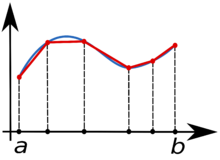
\includegraphics[width=.8\linewidth]{images/trapezium-1.png}
     \caption{Применение составной формулы трапеций}\label{fig:image-1-1-a}
   \end{minipage}\hfill
   \begin{minipage}{0.48\textwidth}
     \centering
     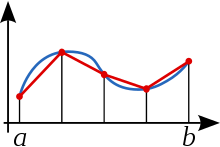
\includegraphics[width=.8\linewidth]{images/trapezium-2.png}
     \caption{Применение формулы трапеций для равномерной сетки}\label{fig:image-1-1-b}
   \end{minipage}
\end{figure}

Если отрезок {{\(\left\lbrack {a,b} \right\rbrack\)}} разбивается узлами
интегрирования {{\(x_{i}\)}}, {{\(i = 0,1,\ldots,n\)}}, так что
{{\(x_{0} = a\)}} и {{\(x_{n} = b\)}}, и на каждом из элементарных
отрезков {{\(\lbrack x_{i},x_{i + 1}\rbrack\)}} применяется формула
трапеций, то суммирование даст \emph{составную формулу трапеций}

\begin{center}
 {{\(\int_{a}^{b}f(x)\, dx \approx \sum\limits_{i = 0}^{n - 1}\frac{f(x_{i}) + f(x_{i + 1})}{2}(x_{i + 1} - x_{i}) =\)}}

{{\(= \frac{f(a)}{2}(x_{1} - a) + \frac{1}{2}\sum\limits_{i = 1}^{n - 1}{f(x_{i})}(x_{i + 1} - x_{i - 1}) + \frac{f(b)}{2}(b - x_{n - 1}).\)}}
\end{center}

\subsubsection{Формула Котеса}

Применение формулы трапеций для равномерной сетки

В случае равномерной сетки {{\(x_{j} = a + jh\)}}, где
{{\(h = (b - a)/n\)}} --- шаг сетки, составная формула трапеций
упрощается:

\begin{center}
 {{\(\int_{a}^{b}f(x)\, dx = h\left( {\frac{f_{0} + f_{n}}{2} + \sum\limits_{i = 1}^{n - 1}f_{i}} \right) + E_{n}(f),\)}}
\end{center}

причём для погрешности справедлива оценка

\begin{center}
 {{\(E_{n}(f) = - \frac{f^{''}(\xi)}{12}(b - a)h^{2}.\)}}
\end{center}

\subsubsection{Свойства}

\begin{itemize}
\item
  Метод трапеций быстро сходится для осциллирующих функций, поскольку
  погрешность за период аннулируется.
\item
  Метод может быть получен путём вычисления среднего арифметического
  между результатами применения формул правых и левых прямоугольников.
\end{itemize}

\subsubsection{Реализация на языке Python}

\lstinputlisting[language=python, frame=single, caption=Метод трапеций на языке Python, tabsize=1, breaklines]{code/listing-5-1.py}

\newpage
\subsection{Метод Симпсона}

\begin{wrapfigure}{l}{0.35\textwidth}
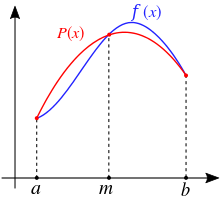
\includegraphics[width=0.9\linewidth]{images/simpson.png}
\caption{\textit{Суть метода — аппроксимация функции $f(x)$ квадратичным полиномом $P(x)$}}
\label{fig:wrapfig}
\end{wrapfigure}

Формула Симпсона (также Ньютона-Симпсона) относится к приёмам численного интегрирования. Получила название в честь британского математика Томаса Симпсона (1710—1761).

Суть метода заключается в приближении подынтегральной функции на отрезке $[a,b]$ интерполяционным многочленом второй степени $p_2(x)$, то есть приближение графика функции на отрезке параболой. Метод Симпсона имеет порядок погрешности 4 и алгебраический порядок точности 3.

\subsubsection{Формула}

Формулой Симпсона называется интеграл от интерполяционного многочлена
второй степени на отрезке {{\(\lbrack a,b\rbrack\)}}:

\begin{center}
 {{\({\int\limits_{a}^{b}f(x)dx} \approx {\int\limits_{a}^{b}{p_{2}(x)}dx} = \frac{b - a}{6}\left( {f(a) + 4f\left( \frac{a + b}{2} \right) + f(b)} \right),\)}}
\end{center}

где {{\(f(a)\)}}, {{\(f((a + b)/2)\)}} и {{\(f(b)\)}}~--- значения
функции в соответствующих точках (на концах отрезка и в его середине).

\subsubsection{Погрешность}

При условии, что у функции {{\(f(x)\)}} на отрезке
{{\(\lbrack a,b\rbrack\)}} существует четвёртая , погрешность
{{\(E(f)\)}}, согласно найденной формуле, равна:

\begin{center}
 {{\(E(f) = - \frac{(b - a)^{5}}{2880}{f^{(4)}(\zeta)},\ \ \ \zeta \in \lbrack a,b\rbrack.\)}}
\end{center}

В связи с тем, что значение {{\(\zeta\)}} зачастую неизвестно, для
оценки погрешности используется следующее неравенство:

\begin{center}
 {{\(\left| {E(f)} \right| \leqslant \frac{(b - a)^{5}}{2880}\max\limits_{x \in \lbrack a,b\rbrack}\left| {f^{(4)}(x)} \right|.\)}}
\end{center}


\subsubsection{Кубаторная формула Симпсона}
Вычисление двойных интегралов также можно свести к формуле Симпсона:

$$
\begin{aligned}
I \approx \frac{h_{x} h_{y}}{9} & \sum_{i=0}^{N-1} \sum_{j=0}^{M-1}\left[f_{2 i, 2 j}+4 f_{2 i+1,2 j}+f_{2 i+2,2 j}+4 f_{2 i, 2 j+1}+16 f_{2 i+1,2 j+1}+\right. \\
& \left.+4 f_{2 i+2,2 j+1}+f_{2 i, 2 j+2}+4 f_{2 i+1,2 j+2}+f_{2 i+2,2 j+2}\right],
\end{aligned}
$$

где $\mathrm{h}_{\mathrm{X}}=(\mathrm{b}-\mathrm{a}) / 2 \mathrm{~N}, \mathrm{hy}=(\mathrm{b}-\mathrm{a}) / 2 \mathrm{M}$.

Если $S$ - криволинейная область интегрирования, то для применения формулы Симпсона область $S$ заключают в прямоугольник $S n(a \leq x \leq b, c \leq y$ $\leq d$ ) и пользуются вспомогательной функцией

$$
g(x,y)={\binom{f(x,y),\ \ \mathrm{emn\\(x,y)\in{\S}},}{\mathrm{emn\\(x,y)\notin{\S}\cdot{\S}}}}.
$$

Тогда

$$
\iint_{(S)} f(x, y) d x d y=\iint_{\left(S_{n}\right)} g(x, y) d x d y
$$

и для вычисления последнего интеграла привлекают метод Симпсона.

\subsubsection{Реализация на языке Python}

\lstinputlisting[language=python, frame=single, caption=Метод Симпсона на языке Python, tabsize=1, breaklines]{code/listing-5-2.py}

\newpage
\subsection{Метод Монте-Карло}

\begin{wrapfigure}{l}{0.45\textwidth}
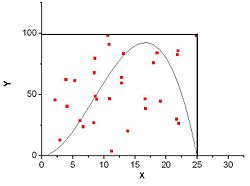
\includegraphics[width=0.9\linewidth]{images/monte_carlo.jpeg}
\caption{\textit{Численное интегрирование функции методом Монте-Карло}}
\label{fig:wrapfig_1}
\end{wrapfigure}

Предположим, необходимо взять интеграл от некоторой функции. Воспользуемся неформальным геометрическим описанием интеграла и будем понимать его как площадь под графиком этой функции.

Для определения этой площади можно воспользоваться одним из обычных численных методов интегрирования: разбить отрезок на подотрезки, подсчитать площадь под графиком функции на каждом из них и сложить. Предположим, что для функции, представленной на рисунке 6, достаточно разбиения на 25 отрезков и, следовательно, вычисления 25 значений функции. Представим теперь, мы имеем дело с $n$-мерной функцией. Тогда нам необходимо $25^n$ отрезков и столько же вычислений значения функции. При размерности функции больше 10 задача становится огромной. Поскольку пространства большой размерности встречаются, в частности, в задачах теории струн, а также многих других физических задачах, где имеются системы со многими степенями свободы, необходимо иметь метод решения, вычислительная сложность которого бы не столь сильно зависела от размерности. Именно таким свойством обладает метод Монте-Карло.

\subsubsection{Алгоритм}

Для определения площади под графиком функции можно использовать
следующий стохастический алгоритм:

\begin{itemize}
\item
  ограничим функцию прямоугольником (\emph{n}-мерным параллелепипедом в
  случае многих измерений), площадь которого {{\(S_{par}\)}} можно легко
  вычислить; \emph{любая сторона прямоугольника содержит хотя бы 1 точку
  графика функции, но не пересекает его;}
\item
  «набросаем» в этот прямоугольник (параллелепипед) некоторое количество
  точек ({{\(N\)}} штук), координаты которых будем выбирать случайным
  образом;
\item
  определим число точек ({{\(K\)}} штук), которые попадут под график
  функции;
\item
  площадь области, ограниченной функцией и осями координат, {{\(S\)}}
  даётся выражением {{\(S = S_{par}\frac{K}{N}\)}}
\end{itemize}

Для малого числа измерений интегрируемой функции производительность
Монте-Карло интегрирования гораздо ниже, чем производительность
детерминированных методов. Тем не менее, в некоторых случаях, когда
функция задана неявно, а необходимо определить область, заданную в виде
сложных неравенств, стохастический метод может оказаться более
предпочтительным.

\subsubsection{Реализация на языке Python}

\lstinputlisting[language=python, frame=single, caption=Метод Монте-Карло на языке Python, tabsize=1, breaklines]{code/listing-5-3.py}

\subsection{Увеличение точности}

Приближение функции одним полиномом на всем отрезке интегрирования, как правило, приводит к большой ошибке в оценке значения интеграла.

Для уменьшения погрешности отрезок интегрирования разбивают на части и применяют численный метод для оценки интеграла на каждой из них.

При стремлении количества разбиений к бесконечности оценка интеграла стремится к его истинному значению для аналитических функций для любого численного метода.

Приведённые выше методы допускают простую процедуру уменьшения шага в два раза, при этом на каждом шаге требуется вычислять значения функции только во вновь добавленных узлах. Для оценки погрешности вычислений используется правило Рунге.

\subsection{Многомерный случай}

В небольших размерностях можно так же применять квадратурные формулы, основанные на интерполяционных многочленах. Интегрирование производится аналогично одномерному интегрированию. Для больших размерностей эти методы становятся неприемлемыми из-за быстрого возрастания числа точек сетки и/или сложной границы области. В этом случае применяется метод Монте-Карло. Генерируются случайные точки в нашей области и усредняются значения функции в них. Так же можно использовать смешанный подход — разбить область на несколько частей, в каждой из которых (или только в тех, где интеграл посчитать не удаётся из-за сложной границы) применить метод Монте-Карло.

\newpage

\begin{center}
 \addsec{Список использованной литературы}
\end{center}

\begin{enumerate}
\item Мулярчик С. Г. Численные методы: Конспект лекций. Мн., БГУ, 2001. 127 с.;
\item И. М. Виноградов. Гаусса метод // Математическая энциклопедия. — М.: Советская энциклопедия. — 1977—1985.
\item Ильин В. А., Позняк Э. Г. Линейная алгебра: Учебник для вузов. — 6-е изд., стер. — М.: ФИЗМАТЛИТ, 2004. — 280 с.
\item Волков Е. А. Численные методы. — М.: Физматлит, 2003.
\item
  {Тихонов А. Н., Самарский
  А. А.} Уравнения математической физики. --- гл.~III
\item  Сальвадори М. Дж. Численные методы в технике. - М., Вузовская книга, 2007.
\end{enumerate}

\end{document}
